\documentclass[aspectratio=169,10pt]{beamer}
\usetheme{Madrid}
\usepackage[utf8]{inputenc}
\usepackage[T1]{fontenc}
\usepackage{listings}
\usepackage{tikz}
\usetikzlibrary{arrows.meta,positioning}
\usepackage{booktabs}
\usepackage{xcolor}

% ---------- Paleta ----------
\definecolor{urAzul}{RGB}{29,53,87}
\definecolor{urTeal}{RGB}{46,125,81}
\definecolor{urGris}{RGB}{90,90,102}
\definecolor{urFondo}{RGB}{240,244,248}
\definecolor{urCode}{RGB}{244,246,248}

\setbeamercolor{palette primary}{bg=urAzul,fg=white}
\setbeamercolor{palette secondary}{bg=urTeal,fg=white}
\setbeamercolor{palette tertiary}{bg=urAzul,fg=white}
\setbeamercolor{frametitle}{bg=urAzul,fg=white}
\setbeamercolor{title}{fg=white}
\setbeamercolor{structure}{fg=urTeal}
\setbeamercolor{block title}{bg=urTeal,fg=white}
\setbeamercolor{block body}{bg=urFondo,fg=black}
\setbeamertemplate{navigation symbols}{}
\setbeamertemplate{itemize item}{\color{urTeal}\textbullet}
\setbeamertemplate{itemize subitem}{\color{urGris}--}

% ---------- Estilo de código SQL ----------
\lstdefinestyle{sql}{
  language=SQL,
  basicstyle=\ttfamily\scriptsize,
  keywordstyle=\color{urAzul}\bfseries,
  commentstyle=\color{urTeal}\itshape,
  stringstyle=\color{urGris},
  backgroundcolor=\color{urCode},
  frame=leftline, framerule=2pt, rulecolor=\color{urTeal},
  numbers=none, showstringspaces=false, breaklines=true,
  xleftmargin=8pt, aboveskip=4pt, belowskip=4pt,
  morekeywords={SERIAL,BOOLEAN,NUMERIC,VARCHAR,TIMESTAMP,REFERENCES,CHECK,UNIQUE,CASCADE,RESTART,IDENTITY,TRUNCATE,generate_series}
}

\title[Base de datos Tienda UR]{Diseño de una base de datos relacional}
\subtitle{Del modelo entidad--relación a las consultas analíticas}
\author[Tienda UR]{E--commerce de la Tienda de Campus}
\institute[UR]{Universidad del Rosario \textperiodcentered\ Ingeniería de Datos}
\date{}

\begin{document}

% ===================== 1. PORTADA =====================
{\setbeamertemplate{footline}{}
\begin{frame}[plain]
  \titlepage
  \begin{center}
    \small\color{urGris}
    Un recorrido metodológico: PostgreSQL, normalización y SQL analítico
  \end{center}
\end{frame}}

% ===================== 2. EL CASO =====================
\begin{frame}{El caso de estudio}
  \begin{block}{Contexto}
    Modelar la tienda de campus de la Universidad, un sistema de comercio
    electrónico al estilo de Amazon o Mercado Libre.
  \end{block}
  \vspace{0.3em}
  \begin{columns}[t]
    \begin{column}{0.32\textwidth}
      \begin{block}{Estudiantes}
        Usuarios con credencial institucional e información de contacto.
      \end{block}
    \end{column}
    \begin{column}{0.32\textwidth}
      \begin{block}{Catálogo}
        Productos organizados por categorías, con precio y disponibilidad.
      \end{block}
    \end{column}
    \begin{column}{0.32\textwidth}
      \begin{block}{Pedidos}
        Flujo completo: carrito, pago y seguimiento de entregas.
      \end{block}
    \end{column}
  \end{columns}
  \vspace{0.4em}
  \begin{center}
    \small\color{urGris}
    Objetivo: \textbf{la menor cantidad de tablas posible}, respetando la normalización.
  \end{center}
\end{frame}

% ===================== 3. HOJA DE RUTA =====================
\begin{frame}{La hoja de ruta}
  \begin{center}
  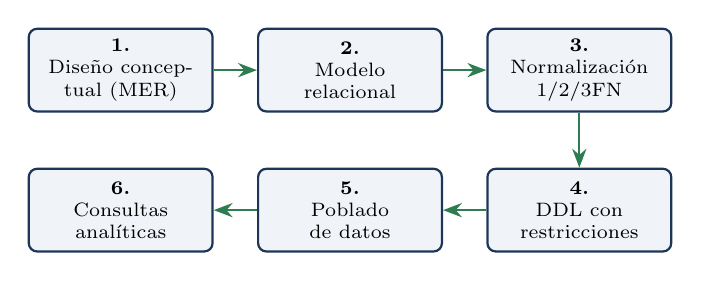
\begin{tikzpicture}[
     nodo/.style={rectangle, rounded corners=3pt, draw=urAzul, thick,
                  fill=urFondo, text width=2.1cm, align=center,
                  minimum height=1.05cm, font=\scriptsize},
     fl/.style={-{Stealth[length=2.4mm]}, urTeal, thick}]
    \node[nodo] (a) {\textbf{1.}\\ Diseño conceptual (MER)};
    \node[nodo, right=0.55cm of a] (b) {\textbf{2.}\\ Modelo relacional};
    \node[nodo, right=0.55cm of b] (c) {\textbf{3.}\\ Normalización 1/2/3FN};
    \node[nodo, below=0.7cm of c] (d) {\textbf{4.}\\ DDL con restricciones};
    \node[nodo, left=0.55cm of d] (e) {\textbf{5.}\\ Poblado de datos};
    \node[nodo, left=0.55cm of e] (f) {\textbf{6.}\\ Consultas analíticas};
    \draw[fl] (a) -- (b);
    \draw[fl] (b) -- (c);
    \draw[fl] (c) -- (d);
    \draw[fl] (d) -- (e);
    \draw[fl] (e) -- (f);
  \end{tikzpicture}
  \end{center}
  \vspace{0.4em}
  \begin{center}
    \small\color{urGris}
    Cada etapa alimenta a la siguiente: del concepto a los datos reales.
  \end{center}
\end{frame}

% ===================== 4a. PASO 0: MER =====================
\begin{frame}{Paso 0 \textbar\ Diseño conceptual (MER)}
  \begin{columns}[t]
    \begin{column}{0.52\textwidth}
      El modelo entidad--relación usa convenciones de forma:
      \begin{itemize}
        \item \textbf{Rectángulo} = entidad
        \item \textbf{Rombo} = relación
        \item \textbf{Óvalo} = atributo (subrayado = llave primaria)
        \item \textbf{1, N, M} = cardinalidad
      \end{itemize}
    \end{column}
    \begin{column}{0.46\textwidth}
      \begin{block}{Cuatro entidades bastan}
        \small
        CLIENTE, CATEGORIA, PRODUCTO y PEDIDO.\\[0.3em]
        La relación \emph{contiene} (pedido--producto) es de muchos a muchos
        y carga atributos propios: cantidad y precio unitario.
      \end{block}
    \end{column}
  \end{columns}
  \vspace{0.3em}
  \begin{center}
    \small\color{urGris}
    En el modelo relacional, ese muchos a muchos se convertirá en una tabla puente.
  \end{center}
\end{frame}

% ===================== 4b. PASO 1: MER (DIAGRAMA CONCEPTUAL) =====================
\begin{frame}{Paso 1 \textbar\ El MER, visualmente}
  \begin{center}
    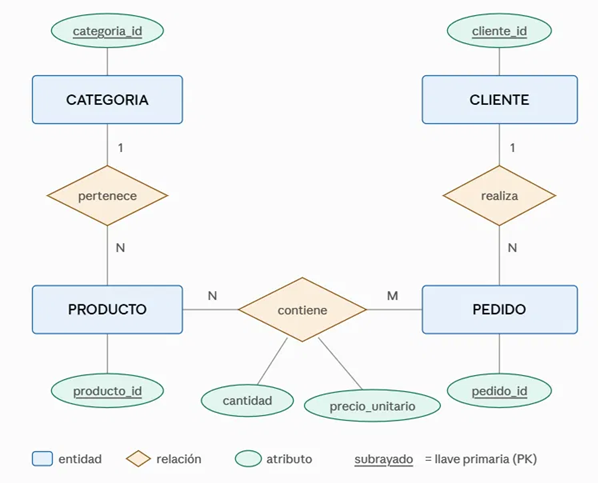
\includegraphics[height=0.80\textheight]{mer_final.png}
  \end{center}
\end{frame}

% ===================== 5. PASO 2: MODELO RELACIONAL (DIAGRAMA) =====================
\begin{frame}{Paso 2 \textbar\ Modelo relacional}
  \begin{center}
    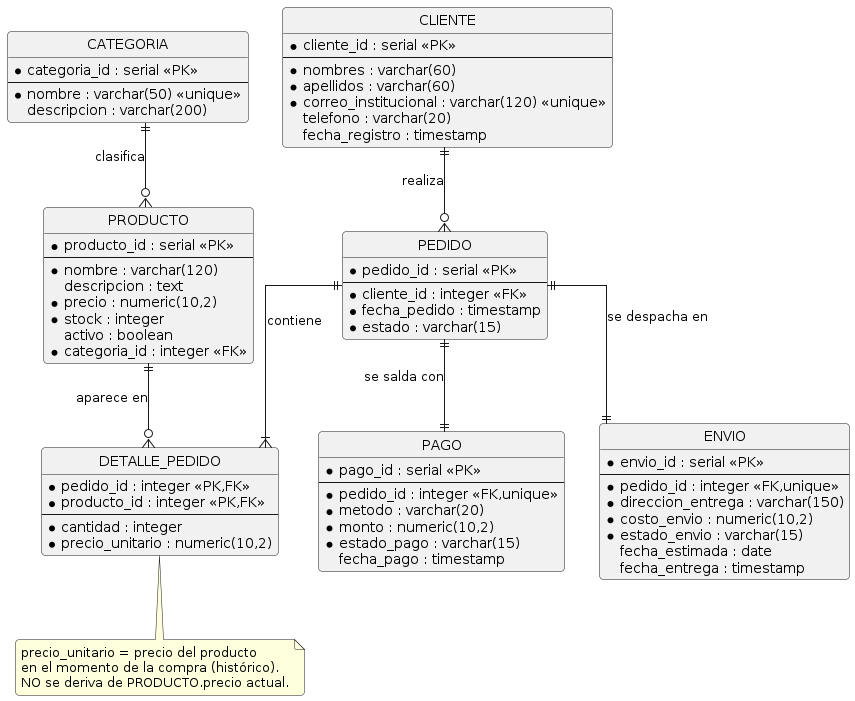
\includegraphics[height=0.82\textheight]{diagrama_final.png}
  \end{center}
\end{frame}

% ===================== 6. PASO 3: NORMALIZACIÓN =====================
\begin{frame}{Paso 3 \textbar\ Normalización}
  \begin{columns}[t]
    \begin{column}{0.33\textwidth}
      \begin{block}{1FN \textemdash\ Atomicidad}
        \small Cada campo guarda un valor único e indivisible. Por eso
        \texttt{nombres} y \texttt{apellidos} van separados.
      \end{block}
    \end{column}
    \begin{column}{0.33\textwidth}
      \begin{block}{2FN \textemdash\ Llave completa}
        \small En \texttt{detalle\_pedido}, cantidad y precio dependen del
        \emph{par} (pedido, producto), no de una parte.
      \end{block}
    \end{column}
    \begin{column}{0.33\textwidth}
      \begin{block}{3FN \textemdash\ Independencia}
        \small El nombre de la categoría vive en su tabla. El total del pedido
        no se almacena: se deriva.
      \end{block}
    \end{column}
  \end{columns}
  \vspace{0.6em}
  \begin{center}
    \small\color{urGris}
    Normalizar aquí significó \textbf{restar} redundancias, no sumar complejidad.
  \end{center}
\end{frame}

% ===================== 7. PASO 4: DDL =====================
\begin{frame}[fragile]{Paso 4 \textbar\ DDL con restricciones}
  Las reglas de negocio se codifican como \texttt{PK}, \texttt{FK}, \texttt{UNIQUE} y \texttt{CHECK}:
  \begin{lstlisting}[style=sql]
CREATE TABLE producto (
  producto_id  SERIAL PRIMARY KEY,
  nombre       VARCHAR(120) NOT NULL,
  precio       NUMERIC(10,2) NOT NULL,
  stock        INTEGER NOT NULL DEFAULT 0,
  categoria_id INTEGER NOT NULL REFERENCES categoria(categoria_id),
  CONSTRAINT chk_precio CHECK (precio >= 0),
  CONSTRAINT chk_stock  CHECK (stock  >= 0)
);
  \end{lstlisting}
  \begin{center}
    \small\color{urGris}
    La base se defiende sola: rechaza cualquier dato que viole las reglas.
  \end{center}
\end{frame}

% ===================== 8. PASO 5: POBLADO =====================
\begin{frame}{Paso 5 \textbar\ Poblado de datos}
  \begin{columns}[t]
    \begin{column}{0.48\textwidth}
      \begin{block}{Tablas base \textemdash\ Mockaroo}
        \small
        Datos realistas para \texttt{cliente} (100) y \texttt{producto} (150),
        exportados a CSV.
      \end{block}
    \end{column}
    \begin{column}{0.48\textwidth}
      \begin{block}{Tablas transaccionales \textemdash\ SQL}
        \small
        \texttt{pedido}, \texttt{detalle\_pedido}, \texttt{pago} y \texttt{envio}
        generados con \texttt{INSERT\ldots SELECT} aleatorio.
      \end{block}
    \end{column}
  \end{columns}
  \vspace{0.5em}
  \begin{center}
    \begin{tabular}{lr}
      \toprule
      \textbf{Tabla} & \textbf{Filas} \\
      \midrule
      categoria & 8 \\
      cliente & 100 \\
      producto & 150 \\
      pedido & 300 \\
      detalle\_pedido & $\approx$900 \\
      pago / envio & 300 / 300 \\
      \bottomrule
    \end{tabular}
  \end{center}
\end{frame}

% ===================== 9. PASO 6: CONSULTAS =====================
\begin{frame}{Paso 6 \textbar\ Consultas analíticas}
  \begin{columns}[t]
    \begin{column}{0.46\textwidth}
      \begin{block}{Ingresos por categoría}
        \small
        \begin{tabular}{lr}
          \toprule
          Categoría & Ingresos \\
          \midrule
          Libros & 16.5\,M \\
          Alimentos y bebidas & 15.9\,M \\
          Regalos y souvenirs & 14.1\,M \\
          Merchandising oficial & 13.5\,M \\
          \bottomrule
        \end{tabular}
      \end{block}
    \end{column}
    \begin{column}{0.50\textwidth}
      \begin{block}{Total de cada pedido}
        \small
        Se calcula al vuelo con \texttt{SUM()}, uniendo pedido, detalle, envío y pago.
        Nunca se almacena: es la \textbf{3FN en acción}.
      \end{block}
      \begin{block}{Otras vistas}
        \small Productos más vendidos, ventas por período, clientes frecuentes.
      \end{block}
    \end{column}
  \end{columns}
\end{frame}

% ===================== 10. CONCLUSIONES =====================
\begin{frame}{Conclusiones}
  \begin{itemize}
    \item Se recorrió el ciclo completo: \textbf{concepto $\rightarrow$ modelo $\rightarrow$ datos $\rightarrow$ análisis}.
    \item Siete tablas normalizadas capturan todo el comercio electrónico sin redundancia.
    \item Las restricciones garantizan la integridad, sin importar cómo entren los datos.
    \item Lo que se puede derivar (el total) \textbf{no se almacena}: se consulta.
  \end{itemize}
  \vfill
  \begin{center}
    \color{urAzul}\large\textbf{Del diagrama a la consulta: un sistema íntegro y consultable.}
  \end{center}
\end{frame}

\end{document}